%%%%%%%%%%%%%%%%%%%%%%%%%%%%%%%%%%%%%%%%%%%%%%%%%%%%%%%%%%%%%%%%%%%%%%%%%%%%%%%%%%%%%%%%%%%%%%%%%%%%%%%%%%%%%%%%%%%%%%
\chapter{Results}
%%%%%%%%%%%%%%%%%%%%%%%%%%%%%%%%%%%%%%%%%%%%%%%%%%%%%%%%%%%%%%%%%%%%%%%%%%%%%%%%%%%%%%%%%%%%%%%%%%%%%%%%%%%%%%%%%%%%%%
!!!!!!!!Hint: kommenter ut bilder, få litt oversikt, og så legg til etterhvert som du går igjennom!!!!!!\\
\section{Convergence}%%%%%%%%%%%%%%%%%%%%%%%%%%%%%%%%%%%%%%%%%%%%%%%%%%%%%%%%%%%%%%%%%%%%%%%%%%%%%%%%%%%%%%%%%%%%%%%%%
This section will show convergence of all the methods, with both Hamiltonian and non-Hamiltonian systems. 

\subsection{Hamiltonain system}%%%%%%%%%%%%%%%%%%%%%%%%%%%%%%%%%%%%%%%%%%%%%%%%%%%%%%%%%%%%%%%%%%%%%%%%%%%%%%%%%%%%%%%
\begin{figure}[H]
        \centering
        \begin{subfigure}[b]{0.30\textwidth}
                \includegraphics[width=\textwidth]{../MATLAB/fig/intconv11.jpg}
                \caption{ Help line decreases with $k^2$. }
                \label{fig:intconvtrap}
        \end{subfigure}
        ~
        \begin{subfigure}[b]{0.30\textwidth}
                \includegraphics[width=\textwidth]{../MATLAB/fig/intconv12.jpg}
                \caption{ Help line decreases with $k$. }
                \label{fig:intconveul}
        \end{subfigure}
        \begin{subfigure}[b]{0.30\textwidth}
                \includegraphics[width=\textwidth]{../MATLAB/fig/intconv13.jpg}
                \caption{ Help line decreases with $k^2$. }
                \label{fig:intconvmid}
        \end{subfigure}
\caption{Figure of the convergence for the different integration methods. All methods converge with the expected rate.}
\label{fig:intconv}
\end{figure}
\subsection{Non-Hamiltonian system}%%%%%%%%%%%%%%%%%%%%%%%%%%%%%%%%%%%%%%%%%%%%%%%%%%%%%%%%%%%%%%%%%%%%%%%%%%%%%%%%%%
\begin{figure}[H]
        \centering
        \begin{subfigure}[b]{0.30\textwidth}
                \includegraphics[width=\textwidth]{../MATLAB/fig/intconv21.jpg}
                %\includegraphics[width=\textwidth]{test}
                \caption{ Help line decreases with $k^2$. }
                \label{fig:intconvtrap2}
        \end{subfigure}
        ~
        \begin{subfigure}[b]{0.30\textwidth}
                \includegraphics[width=\textwidth]{../MATLAB/fig/intconv22.jpg}
                %\includegraphics[width=\textwidth]{test}
                \caption{ Help line decreases with $k$. }
                \label{fig:intconveul2}
        \end{subfigure}
        \begin{subfigure}[b]{0.30\textwidth}
                \includegraphics[width=\textwidth]{../MATLAB/fig/intconv23.jpg}
                %\includegraphics[width=\textwidth]{test}
                \caption{ Help line decreases with $k^2$. }
                \label{fig:intconvmid2}
        \end{subfigure}
\caption{Figure of the convergence for the different integration methods. All methods converge with the expected rate.}
\label{fig:intconv2}
\end{figure}


\section{Integration method} %%%%%%%%%%%%%%%%%%%%%%%%%%%%%%%%%%%%%%%%%%%%%%%%%%%%%%%%%%%%%%%%%%%%%%%%%%%%%%%%%%%
%!!!!!!!!!!!!!!!!Burde det vært restart her også?!!!!!!!!!!!!!!!\\
This section will be concerned with comparing some different methods for integration in time. How well they estimate the error and energy will be the primary concern. \\
!!!!!!!!!!!!!!!!!!!!Her trengs det nye bilder!!!!!!!!!!!!!!!!!!!!!!\\


\subsection{Hamiltonian system}%%%%%%%%%%%%%%%%%%%%%%%%%%%%%%%%%%%%%%%%%%%%%%%%%%%%%%%%%%%%%%%%%%%%%%%%%%%%%%%%%%%%%%%%%%


\begin{figure}[H]
        \centering
        \begin{subfigure}[b]{0.30\textwidth}
                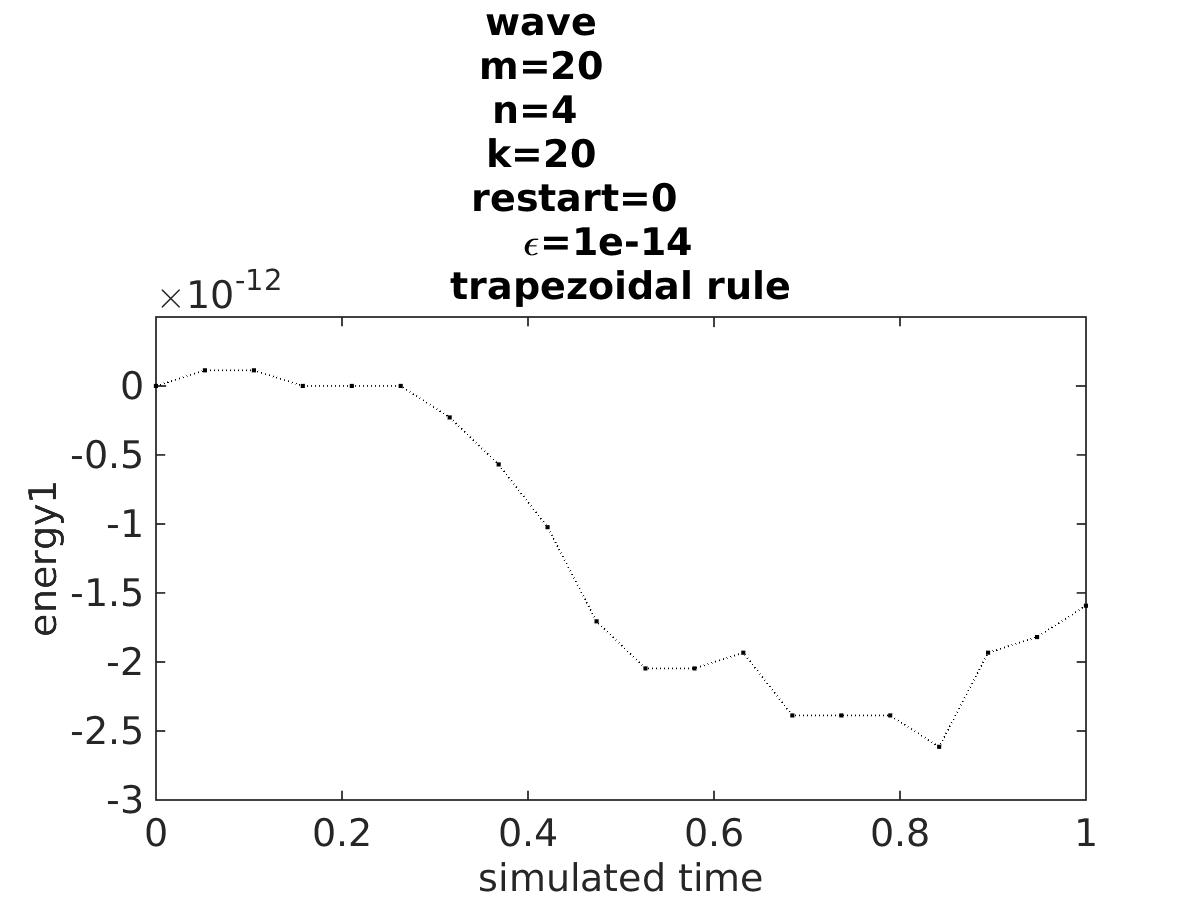
\includegraphics[width=\textwidth]{../MATLAB/fig/energyovertimetrapezoidal.jpg}
                \caption{ Energy with trapezoidal rule. }
                \label{fig:energyovertimetrapezoidal}
        \end{subfigure}%
        ~
        \begin{subfigure}[b]{0.30\textwidth}
                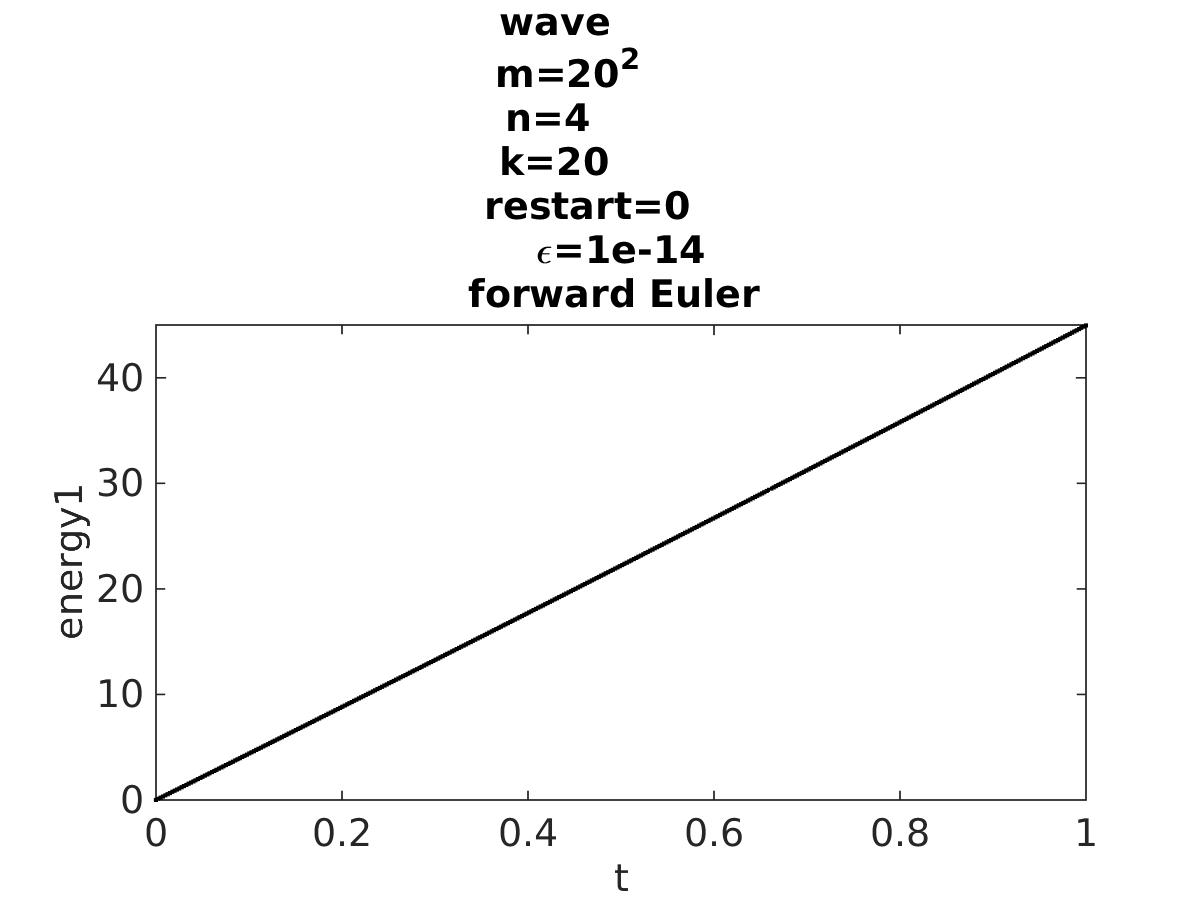
\includegraphics[width=\textwidth]{../MATLAB/fig/energyovertimeeuler.jpg}
                \caption{ Energy with forward Euler }
                \label{fig:energyovertimeeuler}
        \end{subfigure}
        \begin{subfigure}[b]{0.30\textwidth}
                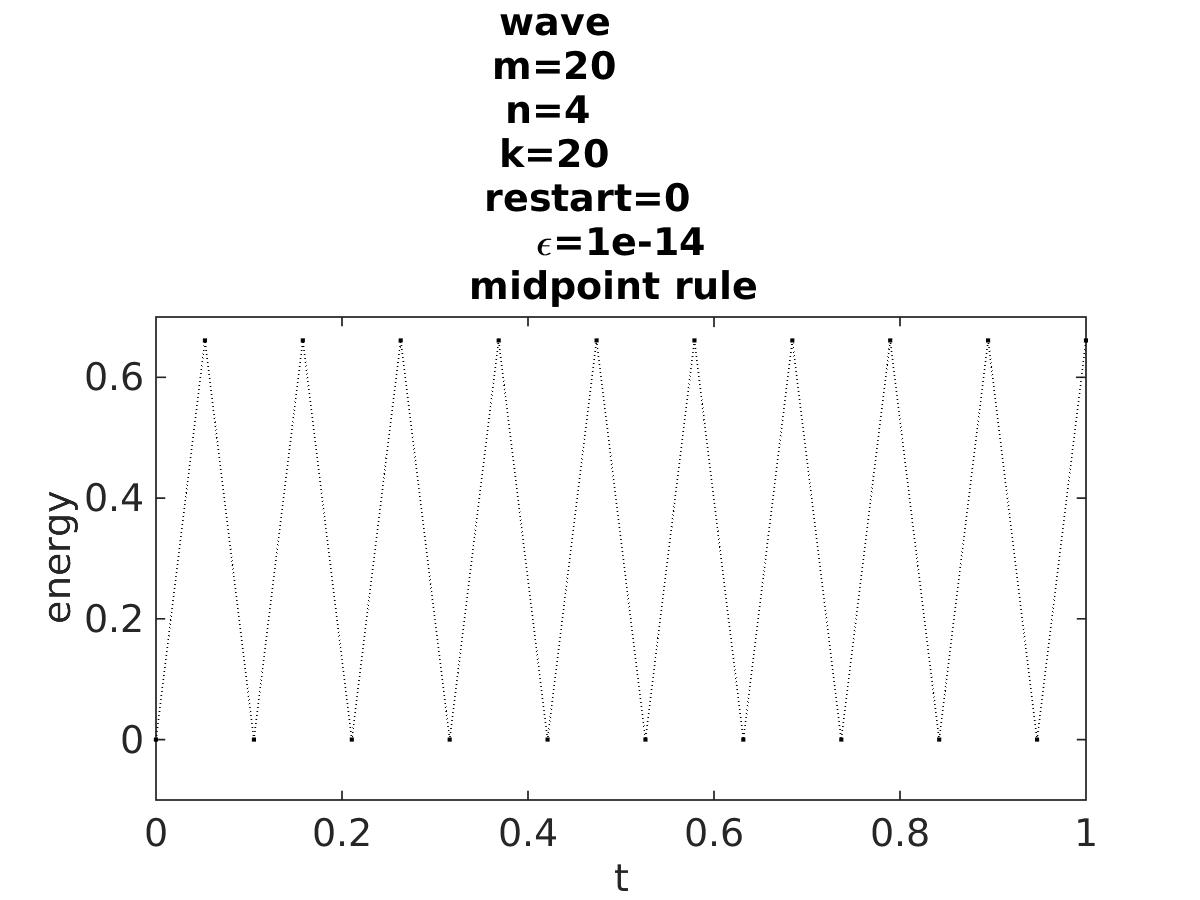
\includegraphics[width=\textwidth]{../MATLAB/fig/energyovertimemidpoint.jpg}
                \caption{ Energy with midpoint rule }
                \label{fig:energyovertimemidpoint}
        \end{subfigure}
        
        \begin{subfigure}[b]{0.30\textwidth}
                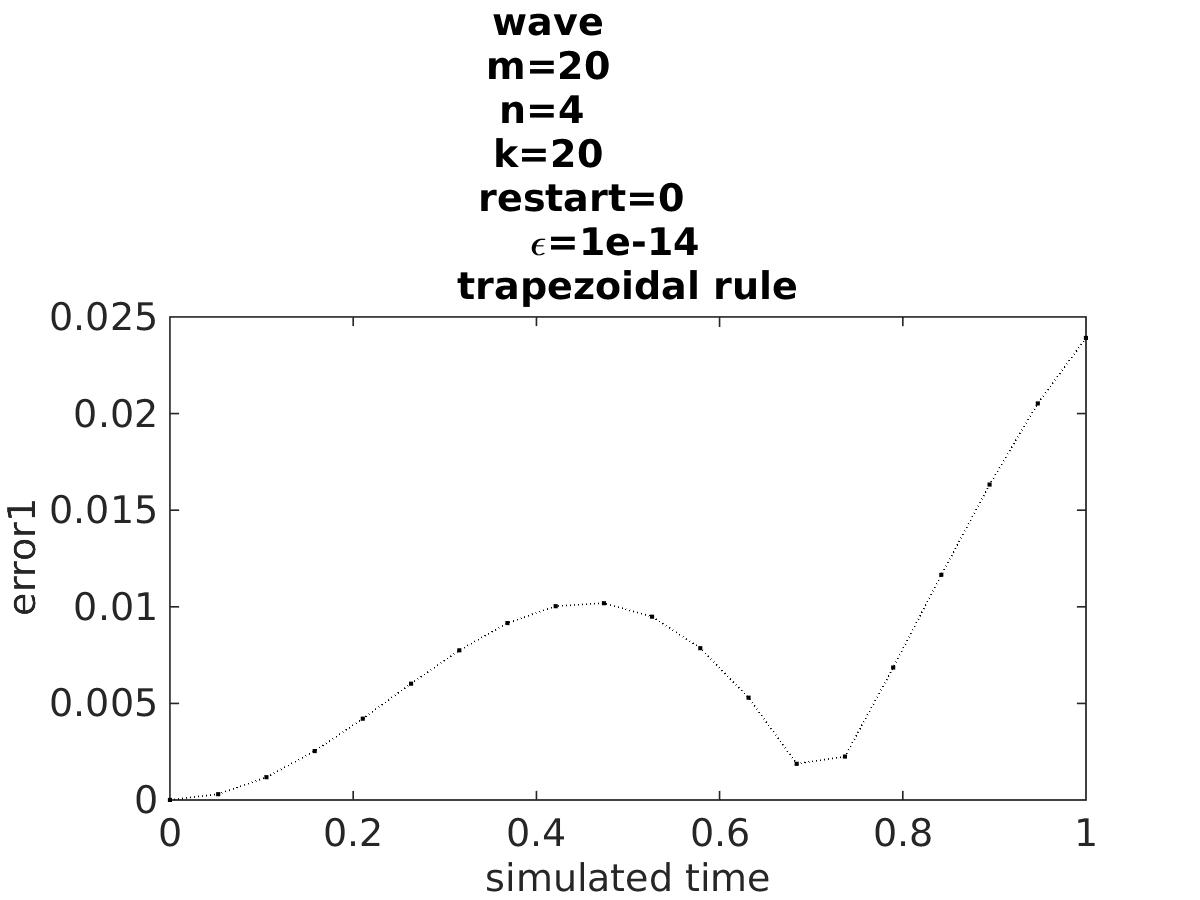
\includegraphics[width=\textwidth]{../MATLAB/fig/errorovertimetrapezoidal.jpg}
                \caption{ Error with trapezoidal rule }
                \label{fig:errorovertimetrapezoidal}
        \end{subfigure}%
        ~
        \begin{subfigure}[b]{0.30\textwidth}
                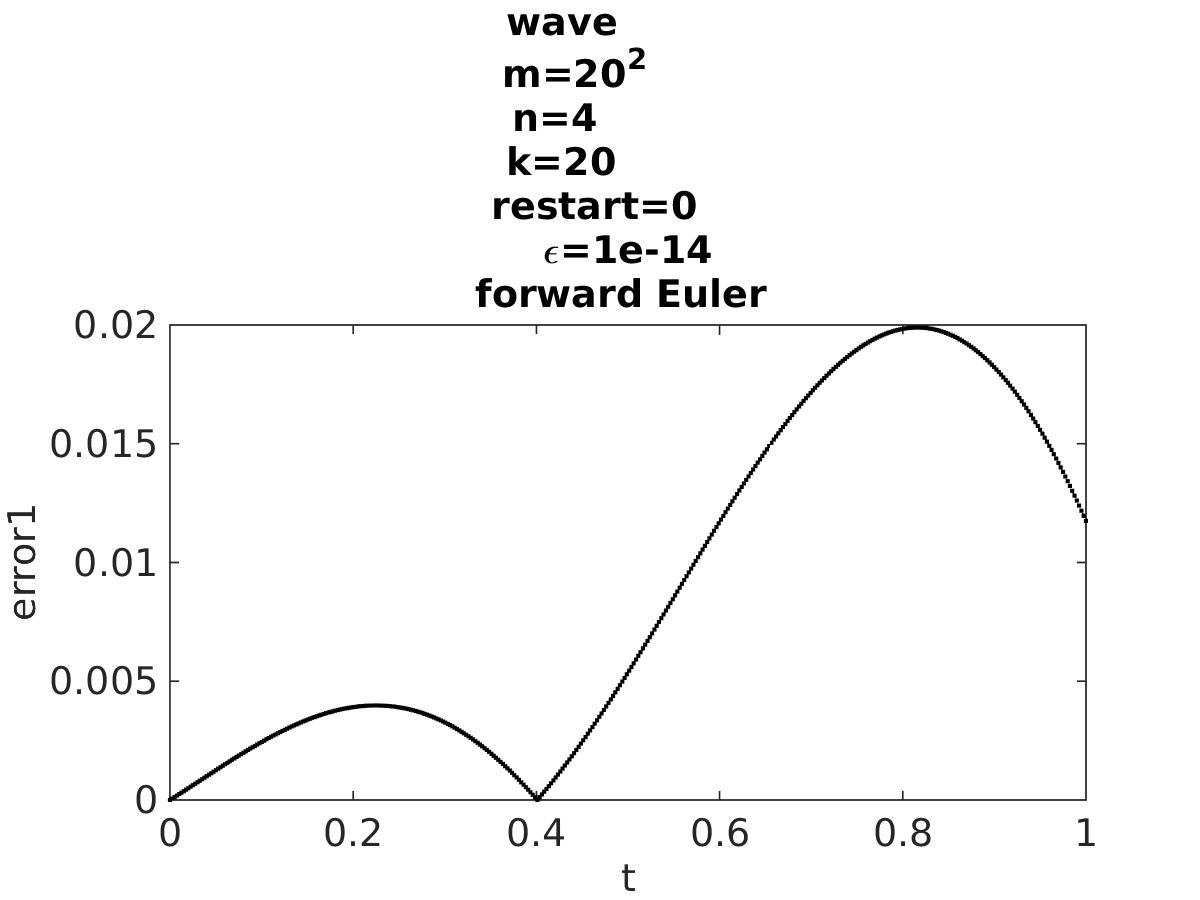
\includegraphics[width=\textwidth]{../MATLAB/fig/errorovertimeeuler.jpg}
                \caption{ Error with forward Euler }
                \label{fig:errorovertimeeuler}
        \end{subfigure}
        \begin{subfigure}[b]{0.30\textwidth}
                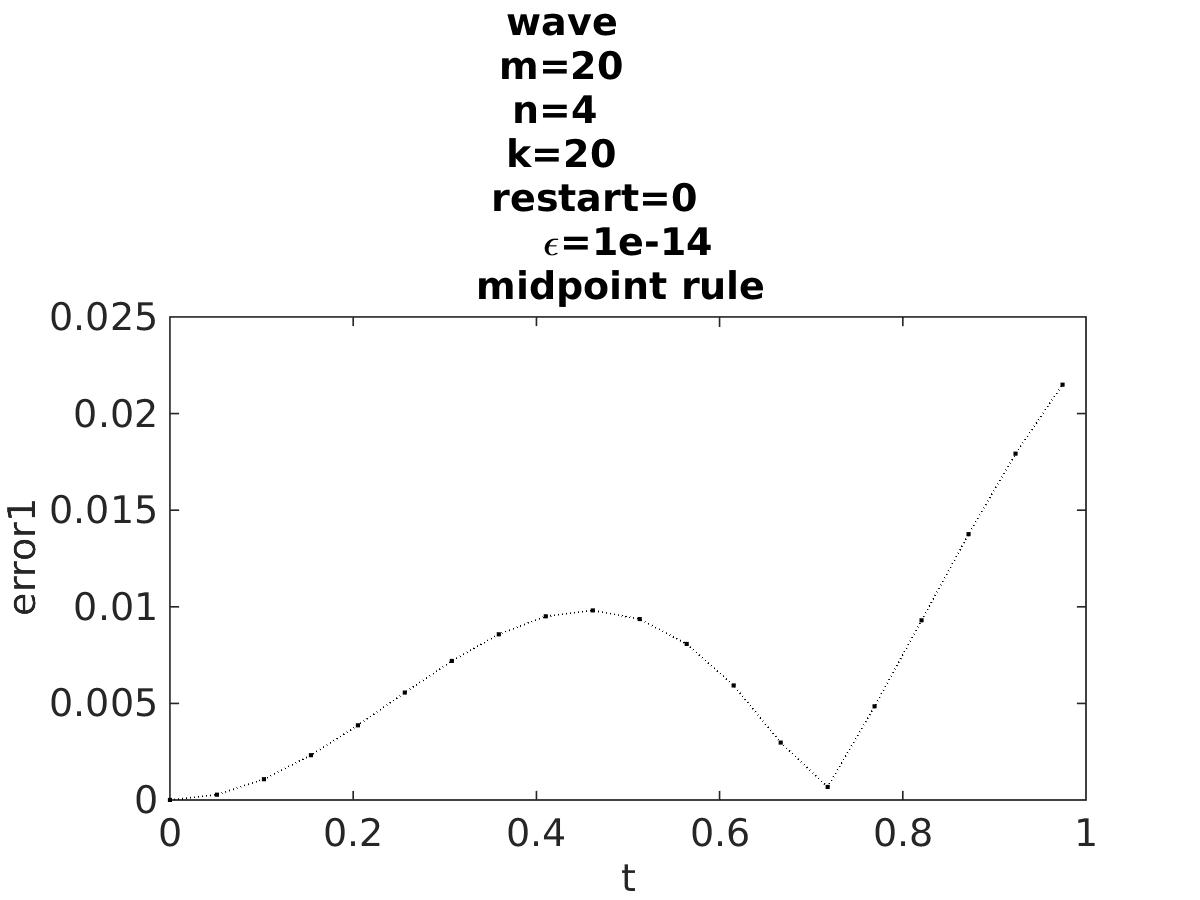
\includegraphics[width=\textwidth]{../MATLAB/fig/errorovertimemidpoint.jpg}
                \caption{ Error with midpoint rule }
                \label{fig:errorovertimemidpoint}
        \end{subfigure}
        \caption{A snapshot of how energy and error changes over the simulated time with the different integration method without restart.}
        \label{fig:error}
\end{figure}
Both trapezoidal rule and midpoint rule to gives a very precise estimation of energy and error. Forward Euler on the other hand gives a linearly increasing energy, and with that a larger error, making it useless as an integration method in this case. The reason for the wired shapes in figure \ref{fig:errorovertimetrapezoidal} and \ref{fig:errorovertimemidpoint} is the periodicity of the test problem. 
\subsection{Non-Hamiltonian system}%%%%%%%%%%%%%%%%%%%%%%%%%%%%%%%%%%%%%%%%%%%%%%%%%%%%%%%%%%%%%%%%%%%%%%%%%%%%%%%%%%%%%%%%%%%

\begin{figure}[H]
        \centering
        \begin{subfigure}[b]{0.30\textwidth}
                \includegraphics[width=\textwidth]{../MATLAB/fig/energychangtimetrapezoidal.jpg}
                \caption{ Energy with trapezoidal rule. }
                \label{fig:energychangtimetrapezoidal}
        \end{subfigure}%
        ~
        \begin{subfigure}[b]{0.30\textwidth}
                \includegraphics[width=\textwidth]{../MATLAB/fig/energychangtimeeuler.jpg}
                \caption{ Energy with forward Euler. }
                \label{fig:energychangtimeeuler}
        \end{subfigure}
        \begin{subfigure}[b]{0.30\textwidth}
                \includegraphics[width=\textwidth]{../MATLAB/fig/energychangtimemidpoint.jpg}
                \caption{ Energy with midpoint rule. }
                \label{fig:energychangtimemidpoint}
        \end{subfigure}
        
        \begin{subfigure}[b]{0.30\textwidth}
                \includegraphics[width=\textwidth]{../MATLAB/fig/errorchangtimetrapezoidal.jpg}
                \caption{ Error with trapezoidal rule. }
                \label{fig:errorchangtimetrapezoidal}
        \end{subfigure}%
        ~
        \begin{subfigure}[b]{0.30\textwidth}
                \includegraphics[width=\textwidth]{../MATLAB/fig/errorchangtimeeuler.jpg}
                \caption{ Error with forward Euler. }
                \label{fig:errorchangtimeeuler}
        \end{subfigure}
        \begin{subfigure}[b]{0.30\textwidth}
                \includegraphics[width=\textwidth]{../MATLAB/fig/errorchangtimemidpoint.jpg}
                \caption{ Error with midpoint rule rule. }
                \label{fig:errorchangtimemidpoint}
        \end{subfigure}
        \caption{A snapshot of how energy and error changes over the simulated time with the different integration method without restart.\\$\neptune$}
        \label{fig:errorchang}
\end{figure}
In this case all methods gives a suitable convergence for the error and the energy. There is no longer any problems with forward Euler's increasing energy. Again the shapes on the figures is a property of the test problems, and not a flaw in the method.

\section{A closer look at SLM }%%%%%%%%%%%%%%%%%%%%%%%%%%%%%%%%%%%%%%%%%%%%%%%%%%%%%%%%%%%%%%%%%%%%%%%%%%%%%%%%%%%%%%%%
%It can be proved that a restart of SLM does not alter the energy \cite{luli}. This section is devoted to seeing holds with numerical approximations. \\

Since SLM gives a symplectic matrix, the energy should not change with time. This section will be devoted to seeing how well this works in practice. There will also be a comparison about how the restart changes the energy preservation. In addition 
!!!!!!!!!!!Bla bla bla!!!!!!!!!!!!!!!!!!!!\\



\subsection{Constant energy} \label{sec:SLMconstant}%%%%%%%%%%%%%%%%%%%%%%%%%%%%%%%%%%%%%%%%%%%%%%%%%%%%%%%%%%%%%%%%%%
!!!!!!!!!!!!!!!!!!!!!Det må skrives en del mer i dette kapitelet!!!!!!!!!!!!!!!!!!!!!!\\

\begin{figure}[H]
        \centering
        \begin{subfigure}[b]{0.3\textwidth}
                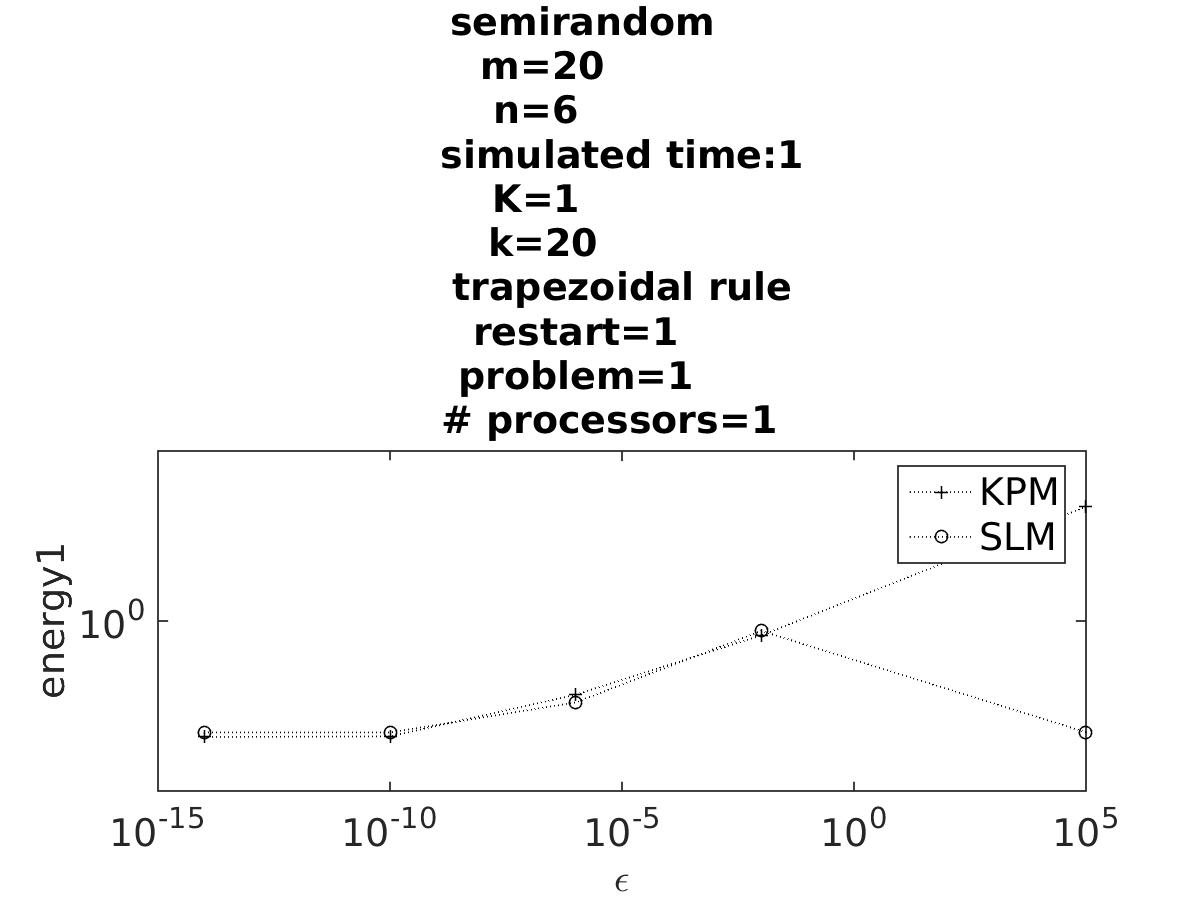
\includegraphics[width=\textwidth]{../MATLAB/fig/compareEnergy.jpg}
                \caption{Energy.}
                \label{fig:compareEnergy}
        \end{subfigure}
        ~
        \begin{subfigure}[b]{0.3\textwidth}
                \includegraphics[width=\textwidth]{../MATLAB/fig/compareError.jpg}
                \caption{ Error. }
                \label{fig:compareError}
        \end{subfigure}
        ~
        \begin{subfigure}[b]{0.3\textwidth}
                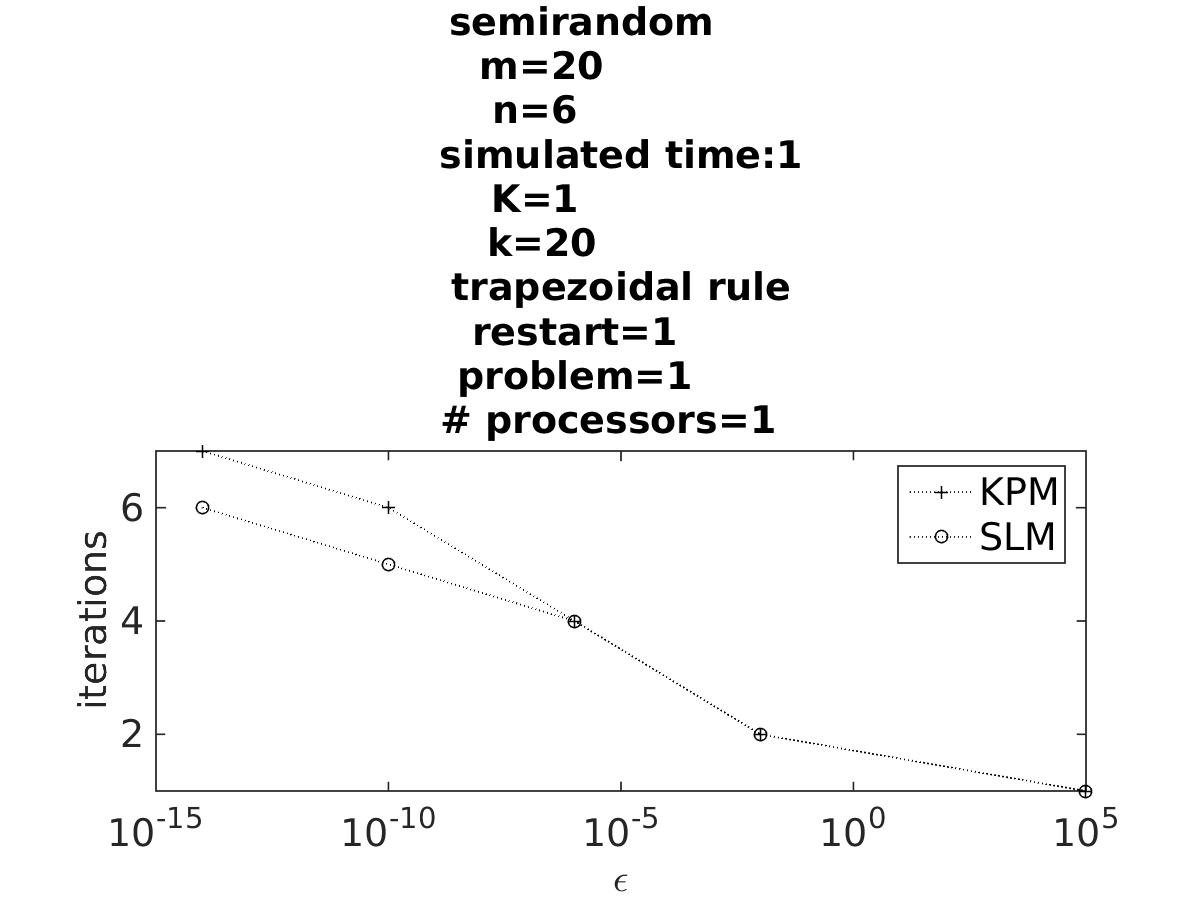
\includegraphics[width=\textwidth]{../MATLAB/fig/compareIter.jpg}
                \caption{ Number of restarts.  }
                \label{fig:compareIter}
        \end{subfigure}
        \caption{ The figure shows how the different methods change the energy and error with different number of restart for \texttt{semirandom}.  }
        \label{fig:compare}
\end{figure}


\begin{figure}[H]
        \centering
        \begin{subfigure}[b]{0.3\textwidth}
                \includegraphics[width=\textwidth]{../MATLAB/fig/compareEnergyw.jpg}
                \caption{ Energy. }
                \label{fig:compareEnergyw}
        \end{subfigure}
        ~
        \begin{subfigure}[b]{0.3\textwidth}
                \includegraphics[width=\textwidth]{../MATLAB/fig/compareErrorw.jpg}
                \caption{ Error. }
                \label{fig:compareErrorw}
        \end{subfigure}
        ~
        \begin{subfigure}[b]{0.3\textwidth}
                \includegraphics[width=\textwidth]{../MATLAB/fig/compareIterw.jpg}
                \caption{ Number of restarts.  }
                \label{fig:compareIterw}
        \end{subfigure}
        \caption{ The figure shows how the different methods change the energy and error with different number of restart for \texttt{wave}.  }
        \label{fig:comparew}
\end{figure}

There is a clear difference between how well the energy is estimated for \texttt{wave} and \texttt{semirandom}. For \texttt{semirandom} there is not much difference between SLM and Arnoldi, although SLM seams to give a slight better approximation than Arnoldi. With \texttt{semirandom} at $\epsilon = 10^{-10}$ Arnoldi preforms one more iteration than SLM, which makes it give a better approximation, aside from that SLM consistently preform better than Arnoldi.\\
When comparing figure \ref{fig:compare} and figure \ref{fig:comparew} it is important to remember that the way the $er_1$ and $er_2$ is found is very differently, and that might explain the why the cases differs so much. But the difference might also be explained with \texttt{semiradom} being a much harder equation to solve.\\
!!!!!!!!!!!!!Skriv litt mer om hvorfor bildene for semirandom og wave er så forksjelkige!!!!!!!!!!!!!!!!!!!!!\\

\subsection{Varying energy}%%%%%%%%%%%%%%%%%%%%%%%%%%%%%%%%%%%%%%%%%%%%%%%%%%%%%%%%%%%%%%%%%%%%%%%%%%%%%%%%%%%%%%%%%%%


\begin{figure}[H]
        \centering
        \begin{subfigure}[b]{0.3\textwidth}
                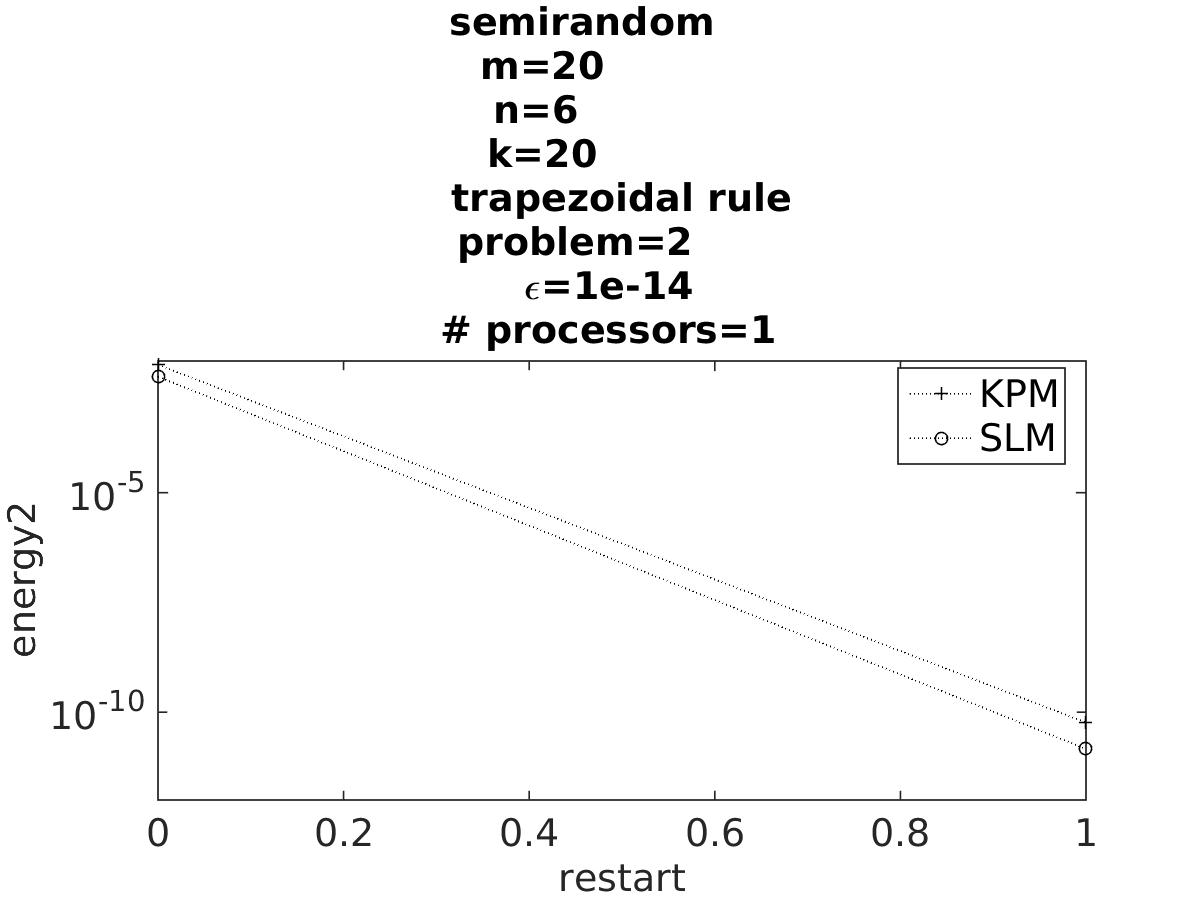
\includegraphics[width=\textwidth]{../MATLAB/fig/compareEnergy2.jpg}
                \caption{ The difference in energy with and without restart. }
                \label{fig:compareEnergy2}
        \end{subfigure}
        ~
        \begin{subfigure}[b]{0.3\textwidth}
                \includegraphics[width=\textwidth]{../MATLAB/fig/compareError2.jpg}
                \caption{ The difference in energy with and without restart. }
                \label{fig:compareError2}
        \end{subfigure}
        ~
        \begin{subfigure}[b]{0.3\textwidth}
                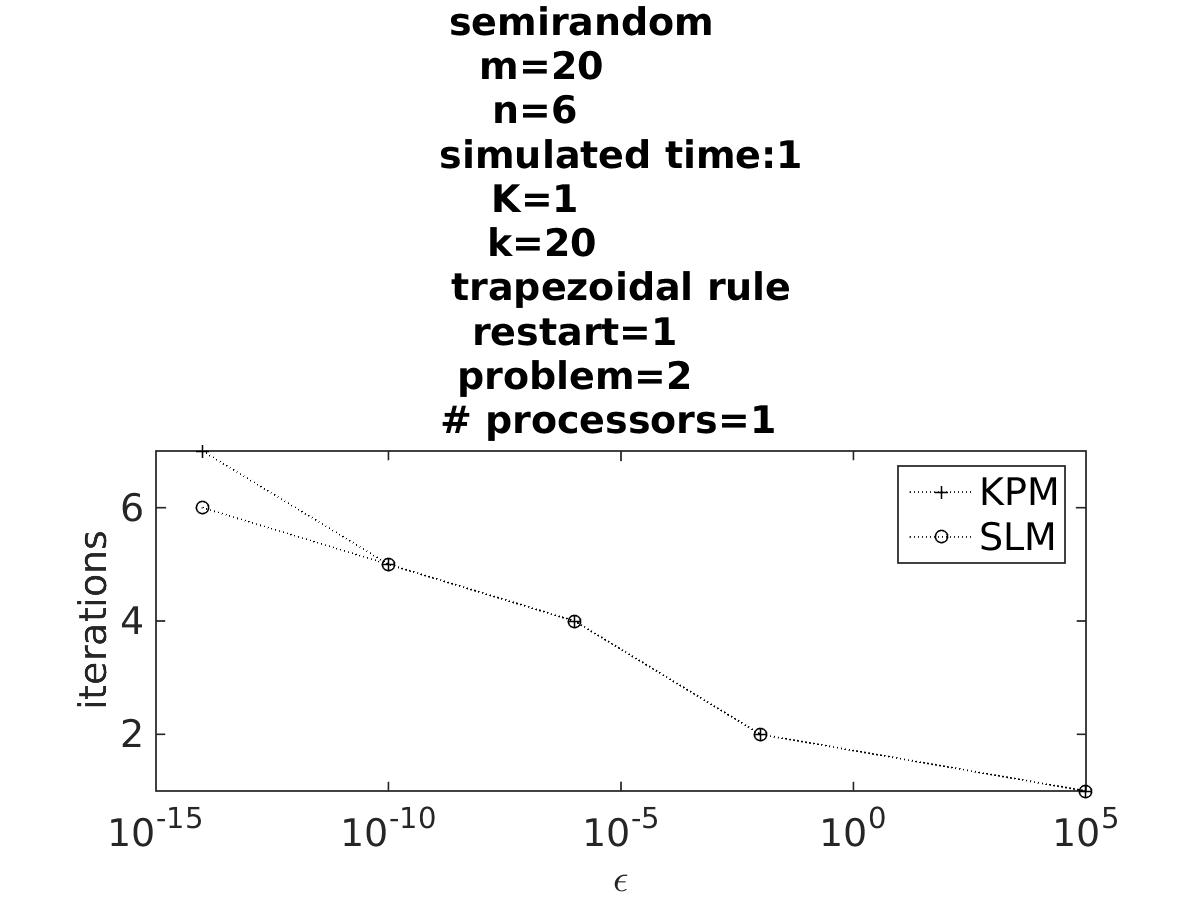
\includegraphics[width=\textwidth]{../MATLAB/fig/compareIter2.jpg}
                \caption{ The number of iterations performed with and without restarting.  }
                \label{fig:compareIter2}
        \end{subfigure}
        \caption{ The figure shows how the different methods change the energy and error with different number of restart for \texttt{wave}.  }
        \label{fig:compare2}
\end{figure}


\begin{figure}[H]
        \centering
        \begin{subfigure}[b]{0.3\textwidth}
                \includegraphics[width=\textwidth]{../MATLAB/fig/compareEnergy2w.jpg}
                \caption{ The difference in energy with and without restart. }
                \label{fig:compareEnergy2w}
        \end{subfigure}
        ~
        \begin{subfigure}[b]{0.3\textwidth}
                \includegraphics[width=\textwidth]{../MATLAB/fig/compareError2w.jpg}
                \caption{ The difference in energy with and without restart. }
                \label{fig:compareError2w}
        \end{subfigure}
        ~
        \begin{subfigure}[b]{0.3\textwidth}
                \includegraphics[width=\textwidth]{../MATLAB/fig/compareIter2w.jpg}
                \caption{ The number of iterations performed with and without restarting.  }
                \label{fig:compareIter2w}
        \end{subfigure}
        \caption{ The figure shows how the different methods change the energy and error with different number of restart for \texttt{wave}.  }
        \label{fig:compare2w}
\end{figure}
The results here are very similar to the results found in section \ref{sec:SLMconstant}, except that the energy and error changes for the first points for both SLM and Arnoldi. SLM still gives the better approximation.

\section{Run time comparison}%%%%%%%%%%%%%%%%%%%%%%%%%%%%%%%%%%%%%%%%%%%%%%%%%%%%%%%%%%%%%%%%%%%%%%%%%%%%%%%%%%%%%%%%%
!!!!!!!!!!!!!!!!!!!!!!!!!!Burde jeg ha med restart eller ikke på disse bildene?!!!!!!!!!!!!!!!!!\\
!!!!!!TEXT!!!!!! \\

\subsection{constant energy}%%%%%%%%%%%%%%%%%%%%%%%%%%%%%%%%%%%%%%%%%%%%%%%%%%%%%%%%%%%%%%%%%%%%%%%%%%%%%%%%%%%%%%%%%%
!!!!!!TEXT!!!!!! 
\begin{figure}[H]
        \centering
        \begin{subfigure}[b]{0.3\textwidth}
                \includegraphics[width=\textwidth]{../MATLAB/fig/ccomparetimem0.jpg}
                \caption{ !!!!!!TEXT!!!!!! }
                \label{fig:ccomparetimem0}
        \end{subfigure}
        ~
        \begin{subfigure}[b]{0.3\textwidth}
                \includegraphics[width=\textwidth]{../MATLAB/fig/ccomparetimem.jpg}
                \caption{ !!!!!!TEXT!!!!!! }
                \label{fig:ccomparetimem}
        \end{subfigure}
        ~

        
        \begin{subfigure}[b]{0.3\textwidth}
                \includegraphics[width=\textwidth]{../MATLAB/fig/ccomparetimek0.jpg}
                \caption{ !!!!!!TEXT!!!!!! }
                \label{fig:ccomparetimek0}
        \end{subfigure}
        ~
        \begin{subfigure}[b]{0.3\textwidth}
                \includegraphics[width=\textwidth]{../MATLAB/fig/ccomparetimek.jpg}
                \caption{ !!!!!!TEXT!!!!!! }
                \label{fig:ccomparetimek}
        \end{subfigure}
        ~

        \caption{ !!!!!!TEXT!!!!!!}
        \label{fig:ccomparetime}
\end{figure}
!!!!!!TEXT!!!!!! \\
\subsection{Varying energy}%%%%%%%%%%%%%%%%%%%%%%%%%%%%%%%%%%%%%%%%%%%%%%%%%%%%%%%%%%%%%%%%%%%%%%%%%%%%%%%%%%%%%%%%%%%
!!!!!!TEXT!!!!!! \\
\begin{figure}[H]
        \centering
        \begin{subfigure}[b]{0.3\textwidth}
                \includegraphics[width=\textwidth]{../MATLAB/fig/vcomparetimem0.jpg}
                \caption{ !!!!!!TEXT!!!!!! }
                \label{fig:vcomparetimem0}
        \end{subfigure}
        ~
        \begin{subfigure}[b]{0.3\textwidth}
                \includegraphics[width=\textwidth]{../MATLAB/fig/vcomparetimem.jpg}
                \caption{ !!!!!!TEXT!!!!!! }
                \label{fig:vcomparetimem}
        \end{subfigure}
        ~

        
        \begin{subfigure}[b]{0.3\textwidth}
                \includegraphics[width=\textwidth]{../MATLAB/fig/vcomparetimek0.jpg}
                \caption{ !!!!!!TEXT!!!!!! }
                \label{fig:vcomparetimek0}
        \end{subfigure}
        ~
        \begin{subfigure}[b]{0.3\textwidth}
                \includegraphics[width=\textwidth]{../MATLAB/fig/vcomparetimek.jpg}
                \caption{ !!!!!!TEXT!!!!!! }
                \label{fig:vcomparetimek}
        \end{subfigure}
        ~

        \caption{ !!!!!!TEXT!!!!!!}
        \label{fig:vcomparetime}
\end{figure}
!!!!!!TEXT!!!!!! \\

\section{Something with slm and energy differnent times}%%%%%%%%%%%%%%%%%%%%%%%%%%%%%%%%%%%%%%%%%%%%%%%%%%%%%%%%%%%%%%
!!!!!!!!!!!!!!!!!Sett dette inn der det hører hjemme!!!!!!!!!!!!!!!!!!!!!!!!!!!!!!!!!!!!!!!!!\\
!!!!!!!Text!!!!!!!!!!!\\

\begin{figure}[H]
        \centering
        \begin{subfigure}[b]{0.3\textwidth}
                \includegraphics[width=\textwidth]{../MATLAB/fig/SLMtimeiter.jpg}
                \caption{ !!!!!!TEXT!!!!!! }
                \label{fig:SLMtimeer1}
        \end{subfigure}
        ~
        \begin{subfigure}[b]{0.3\textwidth}
                \includegraphics[width=\textwidth]{../MATLAB/fig/SLMtimetime.jpg}
                \caption{ !!!!!!TEXT!!!!!! }
                \label{fig:SLMtimeen1}
        \end{subfigure}        
        
        \begin{subfigure}[b]{0.3\textwidth}
                \includegraphics[width=\textwidth]{../MATLAB/fig/SLMtimeer1.jpg}
                \caption{ !!!!!!TEXT!!!!!! }
                \label{fig:SLMtimeer1}
        \end{subfigure}
        ~
        \begin{subfigure}[b]{0.3\textwidth}
                \includegraphics[width=\textwidth]{../MATLAB/fig/SLMtimeen1.jpg}
                \caption{ !!!!!!TEXT!!!!!! }
                \label{fig:SLMtimeen1}
        \end{subfigure}
        
        \begin{subfigure}[b]{0.3\textwidth}
                \includegraphics[width=\textwidth]{../MATLAB/fig/SLMtimeen3.jpg}
                \caption{ !!!!!!TEXT!!!!!! }
                \label{fig:SLMtimeen3}
        \end{subfigure}
        ~
        \begin{subfigure}[b]{0.3\textwidth}
                \includegraphics[width=\textwidth]{../MATLAB/fig/SLMtimeen4.jpg}
                \caption{ !!!!!!TEXT!!!!!! }
                \label{fig:SLMtimeen4}
        \end{subfigure}


        \caption{ !!!!!!TEXT!!!!!!}
        \label{fig:SLMtime}
\end{figure}
!!!!!TEXT!!!!!!!!!!!!!!!\\
\begin{figure}[H]
        \centering
        \begin{subfigure}[b]{0.3\textwidth}
                \includegraphics[width=\textwidth]{../MATLAB/fig/SLMtimeiterf.jpg}
                \caption{ !!!!!!TEXT!!!!!! }
                \label{fig:SLMtimeer1}
        \end{subfigure}
        ~
        \begin{subfigure}[b]{0.3\textwidth}
                \includegraphics[width=\textwidth]{../MATLAB/fig/SLMtimetimef.jpg}
                \caption{ !!!!!!TEXT!!!!!! }
                \label{fig:SLMtimeen1}
        \end{subfigure}        
        
        \begin{subfigure}[b]{0.3\textwidth}
                \includegraphics[width=\textwidth]{../MATLAB/fig/SLMtimeer1f.jpg}
                \caption{ !!!!!!TEXT!!!!!! }
                \label{fig:SLMtimeer1}
        \end{subfigure}
        ~
        \begin{subfigure}[b]{0.3\textwidth}
                \includegraphics[width=\textwidth]{../MATLAB/fig/SLMtimeen1f.jpg}
                \caption{ !!!!!!TEXT!!!!!! }
                \label{fig:SLMtimeen1}
        \end{subfigure}
        
        \begin{subfigure}[b]{0.3\textwidth}
                \includegraphics[width=\textwidth]{../MATLAB/fig/SLMtimeen3f.jpg}
                \caption{ !!!!!!TEXT!!!!!! }
                \label{fig:SLMtimeen3}
        \end{subfigure}
        ~
        \begin{subfigure}[b]{0.3\textwidth}
                \includegraphics[width=\textwidth]{../MATLAB/fig/SLMtimeen4f.jpg}
                \caption{ !!!!!!TEXT!!!!!! }
                \label{fig:SLMtimeen4}
        \end{subfigure}


        \caption{ !!!!!!TEXT!!!!!!}
        \label{fig:SLMtime}
\end{figure}

!!!!!!!Text!!!!!!!!!!!\\
$\mathcal{H}$

\begin{figure}[H]
        \centering
        \begin{subfigure}[b]{0.3\textwidth}
                \includegraphics[width=\textwidth]{../MATLAB/fig/SLMepsilonen3.jpg}
                \caption{ !!!!!!TEXT!!!!!! }
                \label{fig:SLMepsilonen3}
        \end{subfigure}
        ~
        \begin{subfigure}[b]{0.3\textwidth}
                \includegraphics[width=\textwidth]{../MATLAB/fig/SLMepsilonen4.jpg}
                \caption{ !!!!!!TEXT!!!!!! }
                \label{fig:SLMepsilonen4}
        \end{subfigure}
		~
		\begin{subfigure}[b]{0.3\textwidth}
                \includegraphics[width=\textwidth]{../MATLAB/fig/SLMiter.jpg}
                \caption{ !!!!!!TEXT!!!!!! }
                \label{fig:SLMiter}
        \end{subfigure}

        \caption{ !!!!!!TEXT!!!!!!}
        \label{fig:SLMeps}
\end{figure}
